
%% bare_jrnl_compsoc.tex
%% V1.3
%% 2007/01/11
%% by Michael Shell
%% See:
%% http://www.michaelshell.org/
%% for current contact information.
%%
%% This is a skeleton file demonstrating the use of IEEEtran.cls
%% (requires IEEEtran.cls version 1.7 or later) with an IEEE Computer
%% Society journal paper.
%%
%% Support sites:
%% http://www.michaelshell.org/tex/ieeetran/
%% http://www.ctan.org/tex-archive/macros/latex/contrib/IEEEtran/
%% and
%% http://www.ieee.org/

%%*************************************************************************
%% Legal Notice:
%% This code is offered as-is without any warranty either expressed or
%% implied; without even the implied warranty of MERCHANTABILITY or
%% FITNESS FOR A PARTICULAR PURPOSE! 
%% User assumes all risk.
%% In no event shall IEEE or any contributor to this code be liable for
%% any damages or losses, including, but not limited to, incidental,
%% consequential, or any other damages, resulting from the use or misuse
%% of any information contained here.
%%
%% All comments are the opinions of their respective authors and are not
%% necessarily endorsed by the IEEE.
%%
%% This work is distributed under the LaTeX Project Public License (LPPL)
%% ( http://www.latex-project.org/ ) version 1.3, and may be freely used,
%% distributed and modified. A copy of the LPPL, version 1.3, is included
%% in the base LaTeX documentation of all distributions of LaTeX released
%% 2003/12/01 or later.
%% Retain all contribution notices and credits.
%% ** Modified files should be clearly indicated as such, including  **
%% ** renaming them and changing author support contact information. **
%%
%% File list of work: IEEEtran.cls, IEEEtran_HOWTO.pdf, bare_adv.tex,
%%                    bare_conf.tex, bare_jrnl.tex, bare_jrnl_compsoc.tex
%%*************************************************************************

% *** Authors should verify (and, if needed, correct) their LaTeX system  ***
% *** with the testflow diagnostic prior to trusting their LaTeX platform ***
% *** with production work. IEEE's font choices can trigger bugs that do  ***
% *** not appear when using other class files.                            ***
% The testflow support page is at:
% http://www.michaelshell.org/tex/testflow/




% Note that the a4paper option is mainly intended so that authors in
% countries using A4 can easily print to A4 and see how their papers will
% look in print - the typesetting of the document will not typically be
% affected with changes in paper size (but the bottom and side margins will).
% Use the testflow package mentioned above to verify correct handling of
% both paper sizes by the user's LaTeX system.
%
% Also note that the "draftcls" or "draftclsnofoot", not "draft", option
% should be used if it is desired that the figures are to be displayed in
% draft mode.
%
% The Computer Society usually requires 10pt for submissions.
%
\documentclass[10pt,journal,cspaper,compsoc]{IEEEtran}
%
% If IEEEtran.cls has not been installed into the LaTeX system files,
% manually specify the path to it like:
% \documentclass[12pt,journal,compsoc]{../sty/IEEEtran}





% Some very useful LaTeX packages include:
% (uncomment the ones you want to load)


\usepackage{comment} % multi-line comments
\usepackage{graphicx} % necessary for inclusion of .eps for figures
\usepackage{algpseudocode}
\usepackage{amsmath}

\graphicspath{ {./images/} {./gnuplots/} }


% *** MISC UTILITY PACKAGES ***
%
%\usepackage{ifpdf}
% Heiko Oberdiek's ifpdf.sty is very useful if you need conditional
% compilation based on whether the output is pdf or dvi.
% usage:
% \ifpdf
%   % pdf code
% \else
%   % dvi code
% \fi
% The latest version of ifpdf.sty can be obtained from:
% http://www.ctan.org/tex-archive/macros/latex/contrib/oberdiek/
% Also, note that IEEEtran.cls V1.7 and later provides a builtin
% \ifCLASSINFOpdf conditional that works the same way.
% When switching from latex to pdflatex and vice-versa, the compiler may
% have to be run twice to clear warning/error messages.






% *** CITATION PACKAGES ***
%
\ifCLASSOPTIONcompsoc
  % IEEE Computer Society needs nocompress option
  % requires cite.sty v4.0 or later (November 2003)
  % \usepackage[nocompress]{cite}
\else
  % normal IEEE
  % \usepackage{cite}
\fi
% cite.sty was written by Donald Arseneau
% V1.6 and later of IEEEtran pre-defines the format of the cite.sty package
% \cite{} output to follow that of IEEE. Loading the cite package will
% result in citation numbers being automatically sorted and properly
% "compressed/ranged". e.g., [1], [9], [2], [7], [5], [6] without using
% cite.sty will become [1], [2], [5]--[7], [9] using cite.sty. cite.sty's
% \cite will automatically add leading space, if needed. Use cite.sty's
% noadjust option (cite.sty V3.8 and later) if you want to turn this off.
% cite.sty is already installed on most LaTeX systems. Be sure and use
% version 4.0 (2003-05-27) and later if using hyperref.sty. cite.sty does
% not currently provide for hyperlinked citations.
% The latest version can be obtained at:
% http://www.ctan.org/tex-archive/macros/latex/contrib/cite/
% The documentation is contained in the cite.sty file itself.
%
% Note that some packages require special options to format as the Computer
% Society requires. In particular, Computer Society  papers do not use
% compressed citation ranges as is done in typical IEEE papers
% (e.g., [1]-[4]). Instead, they list every citation separately in order
% (e.g., [1], [2], [3], [4]). To get the latter we need to load the cite
% package with the nocompress option which is supported by cite.sty v4.0
% and later. Note also the use of a CLASSOPTION conditional provided by
% IEEEtran.cls V1.7 and later.





% *** GRAPHICS RELATED PACKAGES ***
%
\ifCLASSINFOpdf
  % \usepackage[pdftex]{graphicx}
  % declare the path(s) where your graphic files are
  % \graphicspath{{../pdf/}{../jpeg/}}
  % and their extensions so you won't have to specify these with
  % every instance of \includegraphics
  % \DeclareGraphicsExtensions{.pdf,.jpeg,.png}
\else
  % or other class option (dvipsone, dvipdf, if not using dvips). graphicx
  % will default to the driver specified in the system graphics.cfg if no
  % driver is specified.
  % \usepackage[dvips]{graphicx}
  % declare the path(s) where your graphic files are
  % \graphicspath{{../eps/}}
  % and their extensions so you won't have to specify these with
  % every instance of \includegraphics
  % \DeclareGraphicsExtensions{.eps}
\fi
% graphicx was written by David Carlisle and Sebastian Rahtz. It is
% required if you want graphics, photos, etc. graphicx.sty is already
% installed on most LaTeX systems. The latest version and documentation can
% be obtained at: 
% http://www.ctan.org/tex-archive/macros/latex/required/graphics/
% Another good source of documentation is "Using Imported Graphics in
% LaTeX2e" by Keith Reckdahl which can be found as epslatex.ps or
% epslatex.pdf at: http://www.ctan.org/tex-archive/info/
%
% latex, and pdflatex in dvi mode, support graphics in encapsulated
% postscript (.eps) format. pdflatex in pdf mode supports graphics
% in .pdf, .jpeg, .png and .mps (metapost) formats. Users should ensure
% that all non-photo figures use a vector format (.eps, .pdf, .mps) and
% not a bitmapped formats (.jpeg, .png). IEEE frowns on bitmapped formats
% which can result in "jaggedy"/blurry rendering of lines and letters as
% well as large increases in file sizes.
%
% You can find documentation about the pdfTeX application at:
% http://www.tug.org/applications/pdftex





% *** MATH PACKAGES ***
%
%\usepackage[cmex10]{amsmath}
% A popular package from the American Mathematical Society that provides
% many useful and powerful commands for dealing with mathematics. If using
% it, be sure to load this package with the cmex10 option to ensure that
% only type 1 fonts will utilized at all point sizes. Without this option,
% it is possible that some math symbols, particularly those within
% footnotes, will be rendered in bitmap form which will result in a
% document that can not be IEEE Xplore compliant!
%
% Also, note that the amsmath package sets \interdisplaylinepenalty to 10000
% thus preventing page breaks from occurring within multiline equations. Use:
%\interdisplaylinepenalty=2500
% after loading amsmath to restore such page breaks as IEEEtran.cls normally
% does. amsmath.sty is already installed on most LaTeX systems. The latest
% version and documentation can be obtained at:
% http://www.ctan.org/tex-archive/macros/latex/required/amslatex/math/





% *** SPECIALIZED LIST PACKAGES ***
%
%\usepackage{algorithmic}
% algorithmic.sty was written by Peter Williams and Rogerio Brito.
% This package provides an algorithmic environment fo describing algorithms.
% You can use the algorithmic environment in-text or within a figure
% environment to provide for a floating algorithm. Do NOT use the algorithm
% floating environment provided by algorithm.sty (by the same authors) or
% algorithm2e.sty (by Christophe Fiorio) as IEEE does not use dedicated
% algorithm float types and packages that provide these will not provide
% correct IEEE style captions. The latest version and documentation of
% algorithmic.sty can be obtained at:
% http://www.ctan.org/tex-archive/macros/latex/contrib/algorithms/
% There is also a support site at:
% http://algorithms.berlios.de/index.html
% Also of interest may be the (relatively newer and more customizable)
% algorithmicx.sty package by Szasz Janos:
% http://www.ctan.org/tex-archive/macros/latex/contrib/algorithmicx/




% *** ALIGNMENT PACKAGES ***
%
%\usepackage{array}
% Frank Mittelbach's and David Carlisle's array.sty patches and improves
% the standard LaTeX2e array and tabular environments to provide better
% appearance and additional user controls. As the default LaTeX2e table
% generation code is lacking to the point of almost being broken with
% respect to the quality of the end results, all users are strongly
% advised to use an enhanced (at the very least that provided by array.sty)
% set of table tools. array.sty is already installed on most systems. The
% latest version and documentation can be obtained at:
% http://www.ctan.org/tex-archive/macros/latex/required/tools/


%\usepackage{mdwmath}
%\usepackage{mdwtab}
% Also highly recommended is Mark Wooding's extremely powerful MDW tools,
% especially mdwmath.sty and mdwtab.sty which are used to format equations
% and tables, respectively. The MDWtools set is already installed on most
% LaTeX systems. The lastest version and documentation is available at:
% http://www.ctan.org/tex-archive/macros/latex/contrib/mdwtools/


% IEEEtran contains the IEEEeqnarray family of commands that can be used to
% generate multiline equations as well as matrices, tables, etc., of high
% quality.


%\usepackage{eqparbox}
% Also of notable interest is Scott Pakin's eqparbox package for creating
% (automatically sized) equal width boxes - aka "natural width parboxes".
% Available at:
% http://www.ctan.org/tex-archive/macros/latex/contrib/eqparbox/





% *** SUBFIGURE PACKAGES ***
%\ifCLASSOPTIONcompsoc
%\usepackage[tight,normalsize,sf,SF]{subfigure}
%\else
%\usepackage[tight,footnotesize]{subfigure}
%\fi
% subfigure.sty was written by Steven Douglas Cochran. This package makes it
% easy to put subfigures in your figures. e.g., "Figure 1a and 1b". For IEEE
% work, it is a good idea to load it with the tight package option to reduce
% the amount of white space around the subfigures. Computer Society papers
% use a larger font and \sffamily font for their captions, hence the
% additional options needed under compsoc mode. subfigure.sty is already
% installed on most LaTeX systems. The latest version and documentation can
% be obtained at:
% http://www.ctan.org/tex-archive/obsolete/macros/latex/contrib/subfigure/
% subfigure.sty has been superceeded by subfig.sty.


%\ifCLASSOPTIONcompsoc
%  \usepackage[caption=false]{caption}
%  \usepackage[font=normalsize,labelfont=sf,textfont=sf]{subfig}
%\else
%  \usepackage[caption=false]{caption}
%  \usepackage[font=footnotesize]{subfig}
%\fi
% subfig.sty, also written by Steven Douglas Cochran, is the modern
% replacement for subfigure.sty. However, subfig.sty requires and
% automatically loads Axel Sommerfeldt's caption.sty which will override
% IEEEtran.cls handling of captions and this will result in nonIEEE style
% figure/table captions. To prevent this problem, be sure and preload
% caption.sty with its "caption=false" package option. This is will preserve
% IEEEtran.cls handing of captions. Version 1.3 (2005/06/28) and later 
% (recommended due to many improvements over 1.2) of subfig.sty supports
% the caption=false option directly:
%\ifCLASSOPTIONcompsoc
%  \usepackage[caption=false,font=normalsize,labelfont=sf,textfont=sf]{subfig}
%\else
%  \usepackage[caption=false,font=footnotesize]{subfig}
%\fi
%
% The latest version and documentation can be obtained at:
% http://www.ctan.org/tex-archive/macros/latex/contrib/subfig/
% The latest version and documentation of caption.sty can be obtained at:
% http://www.ctan.org/tex-archive/macros/latex/contrib/caption/




% *** FLOAT PACKAGES ***
%
%\usepackage{fixltx2e}
% fixltx2e, the successor to the earlier fix2col.sty, was written by
% Frank Mittelbach and David Carlisle. This package corrects a few problems
% in the LaTeX2e kernel, the most notable of which is that in current
% LaTeX2e releases, the ordering of single and double column floats is not
% guaranteed to be preserved. Thus, an unpatched LaTeX2e can allow a
% single column figure to be placed prior to an earlier double column
% figure. The latest version and documentation can be found at:
% http://www.ctan.org/tex-archive/macros/latex/base/



%\usepackage{stfloats}
% stfloats.sty was written by Sigitas Tolusis. This package gives LaTeX2e
% the ability to do double column floats at the bottom of the page as well
% as the top. (e.g., "\begin{figure*}[!b]" is not normally possible in
% LaTeX2e). It also provides a command:
%\fnbelowfloat
% to enable the placement of footnotes below bottom floats (the standard
% LaTeX2e kernel puts them above bottom floats). This is an invasive package
% which rewrites many portions of the LaTeX2e float routines. It may not work
% with other packages that modify the LaTeX2e float routines. The latest
% version and documentation can be obtained at:
% http://www.ctan.org/tex-archive/macros/latex/contrib/sttools/
% Documentation is contained in the stfloats.sty comments as well as in the
% presfull.pdf file. Do not use the stfloats baselinefloat ability as IEEE
% does not allow \baselineskip to stretch. Authors submitting work to the
% IEEE should note that IEEE rarely uses double column equations and
% that authors should try to avoid such use. Do not be tempted to use the
% cuted.sty or midfloat.sty packages (also by Sigitas Tolusis) as IEEE does
% not format its papers in such ways.




%\ifCLASSOPTIONcaptionsoff
%  \usepackage[nomarkers]{endfloat}
% \let\MYoriglatexcaption\caption
% \renewcommand{\caption}[2][\relax]{\MYoriglatexcaption[#2]{#2}}
%\fi
% endfloat.sty was written by James Darrell McCauley and Jeff Goldberg.
% This package may be useful when used in conjunction with IEEEtran.cls'
% captionsoff option. Some IEEE journals/societies require that submissions
% have lists of figures/tables at the end of the paper and that
% figures/tables without any captions are placed on a page by themselves at
% the end of the document. If needed, the draftcls IEEEtran class option or
% \CLASSINPUTbaselinestretch interface can be used to increase the line
% spacing as well. Be sure and use the nomarkers option of endfloat to
% prevent endfloat from "marking" where the figures would have been placed
% in the text. The two hack lines of code above are a slight modification of
% that suggested by in the endfloat docs (section 8.3.1) to ensure that
% the full captions always appear in the list of figures/tables - even if
% the user used the short optional argument of \caption[]{}.
% IEEE papers do not typically make use of \caption[]'s optional argument,
% so this should not be an issue. A similar trick can be used to disable
% captions of packages such as subfig.sty that lack options to turn off
% the subcaptions:
% For subfig.sty:
% \let\MYorigsubfloat\subfloat
% \renewcommand{\subfloat}[2][\relax]{\MYorigsubfloat[]{#2}}
% For subfigure.sty:
% \let\MYorigsubfigure\subfigure
% \renewcommand{\subfigure}[2][\relax]{\MYorigsubfigure[]{#2}}
% However, the above trick will not work if both optional arguments of
% the \subfloat/subfig command are used. Furthermore, there needs to be a
% description of each subfigure *somewhere* and endfloat does not add
% subfigure captions to its list of figures. Thus, the best approach is to
% avoid the use of subfigure captions (many IEEE journals avoid them anyway)
% and instead reference/explain all the subfigures within the main caption.
% The latest version of endfloat.sty and its documentation can obtained at:
% http://www.ctan.org/tex-archive/macros/latex/contrib/endfloat/
%
% The IEEEtran \ifCLASSOPTIONcaptionsoff conditional can also be used
% later in the document, say, to conditionally put the References on a 
% page by themselves.




% *** PDF, URL AND HYPERLINK PACKAGES ***
%
%\usepackage{url}
% url.sty was written by Donald Arseneau. It provides better support for
% handling and breaking URLs. url.sty is already installed on most LaTeX
% systems. The latest version can be obtained at:
% http://www.ctan.org/tex-archive/macros/latex/contrib/misc/
% Read the url.sty source comments for usage information. Basically,
% \url{my_url_here}.





% *** Do not adjust lengths that control margins, column widths, etc. ***
% *** Do not use packages that alter fonts (such as pslatex).         ***
% There should be no need to do such things with IEEEtran.cls V1.6 and later.
% (Unless specifically asked to do so by the journal or conference you plan
% to submit to, of course. )


% correct bad hyphenation here
\hyphenation{op-tical net-works semi-conduc-tor}


\begin{document}
%
% paper title
% can use linebreaks \\ within to get better formatting as desired
\title{Markov Models of Leader Elections in a Smart Grid System}
%
%
% author names and IEEE memberships
% note positions of commas and nonbreaking spaces ( ~ ) LaTeX will not break
% a structure at a ~ so this keeps an author's name from being broken across
% two lines.
% use \thanks{} to gain access to the first footnote area
% a separate \thanks must be used for each paragraph as LaTeX2e's \thanks
% was not built to handle multiple paragraphs
%
%
%\IEEEcompsocitemizethanks is a special \thanks that produces the bulleted
% lists the Computer Society journals use for "first footnote" author
% affiliations. Use \IEEEcompsocthanksitem which works much like \item
% for each affiliation group. When not in compsoc mode,
% \IEEEcompsocitemizethanks becomes like \thanks and
% \IEEEcompsocthanksitem becomes a line break with idention. This
% facilitates dual compilation, although admittedly the differences in the
% desired content of \author between the different types of papers makes a
% one-size-fits-all approach a daunting prospect. For instance, compsoc 
% journal papers have the author affiliations above the "Manuscript
% received ..."  text while in non-compsoc journals this is reversed. Sigh.

\author{Stephen~Jackson,~\IEEEmembership{Student Member,~IEEE}
        Bruce~McMillin,~\IEEEmembership{Senior Member,~IEEE}%<--??
\IEEEcompsocitemizethanks{\IEEEcompsocthanksitem S. Jackson and B. McMillin are with the Department
of Computer Science, Missouri University of Science \& Technology, Rolla,
MO, 65409.\protect\\
% note need leading \protect in front of \\ to get a newline within \thanks as
% \\ is fragile and will error, could use \hfil\break instead.
E-mail: scj7t4@mst.edu, ff@mst.edu}
\thanks{}}

% note the % following the last \IEEEmembership and also \thanks - 
% these prevent an unwanted space from occurring between the last author name
% and the end of the author line. i.e., if you had this:
% 
% \author{....lastname \thanks{...} \thanks{...} }
%                     ^------------^------------^----Do not want these spaces!
%
% a space would be appended to the last name and could cause every name on that
% line to be shifted left slightly. This is one of those "LaTeX things". For
% instance, "\textbf{A} \textbf{B}" will typeset as "A B" not "AB". To get
% "AB" then you have to do: "\textbf{A}\textbf{B}"
% \thanks is no different in this regard, so shield the last } of each \thanks
% that ends a line with a % and do not let a space in before the next \thanks.
% Spaces after \IEEEmembership other than the last one are OK (and needed) as
% you are supposed to have spaces between the names. For what it is worth,
% this is a minor point as most people would not even notice if the said evil
% space somehow managed to creep in.



% The paper headers
\markboth{Journal of \LaTeX\ Class Files,~Vol.~6, No.~1, January~2007}%
{Shell \MakeLowercase{\textit{et al.}}: Bare Demo of IEEEtran.cls for Computer Society Journals}
% The only time the second header will appear is for the odd numbered pages
% after the title page when using the twoside option.
% 
% *** Note that you probably will NOT want to include the author's ***
% *** name in the headers of peer review papers.                   ***
% You can use \ifCLASSOPTIONpeerreview for conditional compilation here if
% you desire.



% The publisher's ID mark at the bottom of the page is less important with
% Computer Society journal papers as those publications place the marks
% outside of the main text columns and, therefore, unlike regular IEEE
% journals, the available text space is not reduced by their presence.
% If you want to put a publisher's ID mark on the page you can do it like
% this:
%\IEEEpubid{0000--0000/00\$00.00~\copyright~2007 IEEE}
% or like this to get the Computer Society new two part style.
%\IEEEpubid{\makebox[\columnwidth]{\hfill 0000--0000/00/\$00.00~\copyright~2007 IEEE}%
%\hspace{\columnsep}\makebox[\columnwidth]{Published by the IEEE Computer Society\hfill}}
% Remember, if you use this you must call \IEEEpubidadjcol in the second
% column for its text to clear the IEEEpubid mark (Computer Society jorunal
% papers don't need this extra clearance.)




% for Computer Society papers, we must declare the abstract and index terms
% PRIOR to the title within the \IEEEcompsoctitleabstractindextext IEEEtran
% command as these need to go into the title area created by \maketitle.
\IEEEcompsoctitleabstractindextext{%
\begin{abstract}
%\boldmath
Cyber-physical systems are an attractive option for future development of
critical infrastructure systems. By supplementing the traditional physical
network with cyber control, the performance and reliability of the system
can be increased. In some of these networks, distributing the cyber control
offers increased redundancy and availability during fault conditions. However,
there are very few works which study the effects of cyber faults on a 
distributed cyber-physical system. These are of a particular interest in the Smart Grid
environment where outages and failures are very costly. By examining the
behavior of a distributed system under fault scenarios, the overall robustness
of the system can be improved by planning characteristics and responses to
faults that allow the system to continue operating in difficult circumstances. 
\end{abstract}
% IEEEtran.cls defaults to using nonbold math in the Abstract.
% This preserves the distinction between vectors and scalars. However,
% if the journal you are submitting to favors bold math in the abstract,
% then you can use LaTeX's standard command \boldmath at the very start
% of the abstract to achieve this. Many IEEE journals frown on math
% in the abstract anyway. In particular, the Computer Society does
% not want either math or citations to appear in the abstract.

% Note that keywords are not normally used for peer review papers.
\begin{keywords}
Distributed Computing, Smart Grid, Leader Election, Group Management, Reliability, Robustness
\end{keywords}}


% make the title area
\maketitle


% To allow for easy dual compilation without having to reenter the
% abstract/keywords data, the \IEEEcompsoctitleabstractindextext text will
% not be used in maketitle, but will appear (i.e., to be "transported")
% here as \IEEEdisplaynotcompsoctitleabstractindextext when compsoc mode
% is not selected <OR> if conference mode is selected - because compsoc
% conference papers position the abstract like regular (non-compsoc)
% papers do!
\IEEEdisplaynotcompsoctitleabstractindextext
% \IEEEdisplaynotcompsoctitleabstractindextext has no effect when using
% compsoc under a non-conference mode.


% For peer review papers, you can put extra information on the cover
% page as needed:
% \ifCLASSOPTIONpeerreview
% \begin{center} \bfseries EDICS Category: 3-BBND \end{center}
% \fi
%
% For peerreview papers, this IEEEtran command inserts a page break and
% creates the second title. It will be ignored for other modes.
\IEEEpeerreviewmaketitle



\section{Introduction}
% Computer Society journal papers do something a tad strange with the very
% first section heading (almost always called "Introduction"). They place it
% ABOVE the main text! IEEEtran.cls currently does not do this for you.
% However, You can achieve this effect by making LaTeX jump through some
% hoops via something like:
%
%\ifCLASSOPTIONcompsoc
%  \noindent\raisebox{2\baselineskip}[0pt][0pt]%
%  {\parbox{\columnwidth}{\section{Introduction}\label{sec:introduction}%
%  \global\everypar=\everypar}}%
%  \vspace{-1\baselineskip}\vspace{-\parskip}\par
%\else
%  \section{Introduction}\label{sec:introduction}\par
%\fi
%
% Admittedly, this is a hack and may well be fragile, but seems to do the
% trick for me. Note the need to keep any \label that may be used right
% after \section in the above as the hack puts \section within a raised box.



% The very first letter is a 2 line initial drop letter followed
% by the rest of the first word in caps (small caps for compsoc).
% 
% form to use if the first word consists of a single letter:
% \IEEEPARstart{A}{demo} file is ....
% 
% form to use if you need the single drop letter followed by
% normal text (unknown if ever used by IEEE):
% \IEEEPARstart{A}{}demo file is ....
% 
% Some journals put the first two words in caps:
% \IEEEPARstart{T}{his demo} file is ....
% 
% Here we have the typical use of a "T" for an initial drop letter
% and "HIS" in caps to complete the first word.
\IEEEPARstart{F}{REEDM} (Future Renewable Electric Energy Delivery and Management) System
is a Smart Grid project focused on the future of the electrical grid. Major proposed features
of the FREEDM network include the Solid State Transformer, distributed local energy storage,
and distributed local energy generation\cite{FREEDMMIGRATION}. This vein of research emphasizes decentralizing the
power grid: making it more reliable by distributing energy production resources. Part of this
design requires the system to operate in islanded mode, where portions of the distribution
network are segmented from each other.

The effects of these partitions are still not well understood, especially since in a distributed
cyber-physical system partitions may occur in both the cyber and physical domains. As a result,
it is not well known how cyber or physical fault will effect the other portion of the system.
However, research such as \cite{HARINI}\cite{TSG}, indicates that cyber faults can cause a
physical system apply unstable settings.

This work presents the initial steps to better understanding and planning for these faults.
By taking a new approach to considering how a distributed system interacts during a fault condition,
new techniques for managing a fault scenario in a cyber-physical systems will be created. To do
this, we present an approach in modeling the grouping behavior of a system using Markov chains.
These chains produce expectations of how long a system can be expected to stay in a particular
state, or how much time it will be able to spend coordinating and doing useful work over a period
of time. Using these measures, the behavior of the control system for the physical devices 
can be adjusted to prevent faults.

The next section describes the FREEDM smart-grid system and the DGI (Distributed Grid Intelligence). In section 3,
we overview the group management algorithm, and the state of the art for distributed
systems. In section 4 we describe in detail the architecture of the DGI, including the architecture
of the message passing interface and the protocols used in the experiments, as well as our
experimental setup. In section 5 we outline our previous results, collected by running the DGI
in a controlled environment. Section 6 explains the assumptions and how the Markov Chains are
contructed. In section 7, we show the accuracy of these models for predicting grouping behavior
of the system. Conclusions are presented in the final section.

%\IEEEpubidadjcol
% needed in second column of first page if using \IEEEpubid
\section{FREEDM DGI}
In this work we model the group management module of the FREEDM DGI (Distributed Grid Intelligence).
The DGI (Distributed Grid Intelligence) is a smart grid operating system
that organizes and coordinates power electronics and negotiates contracts to
deliver power to devices and regions that cannot effectively facilitate their own need.
The DGI leverages common distributed algorithms to control the power grid, making it an
attractive target for modelling a distributed system.

(Is one sentence enough to smooth that over? I'm struggling a bit with smoothing that out)

To accomplish this, the DGI software consists of a central component, the
broker, which is responsible for presenting a communication interface and
furnishing any common functionality needed by any algorithms used by the
system. These algorithms are grouped into modules. These algorithms work in
concert to move power from areas of excess supply to excess demand.

The DGI uses several modules to manage a distributed smart-grid system. Group
management, the focus of this work, implements a leader election algorithm to
discover which nodes are reachable in the cyber domain.

Other modules provide additional functionality such as collecting global
snapshots, and a module that negotiates the migrations and gives commands to
physical components.

The DGI is a real-time system: certain actions (and reactions) involving power
system components need to be completed with a pre-specified time-frame to keep
the system stable. The DGI uses a round robin scheduler: each module is given
a predetermined window of execution which it may use to perform its duties. When
a module's time period expires, the next module in the line is allowed to
execute. 
 
\section{Group Management}
The DGI uses the leader election algorithm, ``Invitation Election
Algorithm'' written by Garcia-Molina in \cite{INVITATIONELECTION}.
Originally published in 1982, his algorithm provides a robust election 
procedure which allows for transient
partitions. Transient partitions are formed when a faulty link between two or
more clusters of DGIs causes the groups to temporarily divide. These transient
partitions merge when the link is more reliable. The election algorithm
allows for failures that disconnect two distinct sub-networks. These sub
networks are fully connected, but connectivity between the two sub-networks is
limited by an unreliable link.

Since Garcia-Molina's original publication, there has been a large body of
work creating various election algorithms. Each algorithm is
designed to be well suited to the circumstances it will deployed in: there are
specialized algorithms for wireless sensor
networks\cite{LE-WSN-1}\cite{LE-WSN-2}, detecting failures in
certain
circumstances\cite{LE-SPECIALCIRCUMSTANCES-1}\cite{LE-SPECIALCIRCUMSTANCES-2}, and of course, transient partitions. Work on leader
elections has been incorporated into a variety of distributed frameworks:
Isis\cite{ISISTOOLKIT},
Horus\cite{HORUSTOOLKIT}, Totem\cite{TOTEMTOOLKIT},
Transis\cite{TRANSISTOOLKIT}, and Spread\cite{SPREADTOOLKIT} all have methods for creating groups. Despite
this wide body of work, the fundamentals of leader election are consistent
across all work: nodes arrive at a consensus of a single peer who coordinates
the group, and nodes the fail are detected and removed from the group. 

The elected leader is responsible for making work assignments and identifying
and merging with other coordinators when they are found, as well as maintaining
an up-to-date list of peers for the members of his group.  Likewise, members of
the group can detect the failure of the group leader by periodically checking
if the group leader is still alive by sending a message. If the leader fails to
respond, the querying nodes will enter a recovery state and operate alone until
they can identify another coordinator to join with. Therefore, a leader and each
of the members maintains a set of processes which are currently reachable, which
is a subset of all known processes in the system.

This Leader election can also be classified as a failure detector
\cite{LEADERELECTIONEVAL}. Failure detectors are algorithms which detect the failure of processes in a
system. A failure detector algorithm maintains a list of processes that it suspects have
crashed. This informal description gives the failure detector strong ties to the
Leader Election process. The Group Management module maintains a list of
suspected processes which can be determined from the set of all processes and the current
membership.

The leader and members have separate roles to play in the failure detection
process. Leaders use a periodic search to locate other leaders in order to merge groups.
 This serves as a ping / response query for
detecting failures in the system. It is also capable of detecting a change in state either
by network issue or crash failure that causes the process being queried to no
longer consider itself part of the leader's group. The member will only suspect the leader, and not the other processes.
Of course, simple modifications could allow the member to suspect other members
by use of a heart beat or query-reply system, but it is not implemented in DGI code.

In this work it is assumed that a leader does not span two partitioned networks:
if a group is able to form, all members have some chance of communicating with
each other.

\section {Experimental Setup}

\subsection{Broker Architecture}
The DGI software is designed around a broker architectural specification.
Each core functionality of the system is implemented within a module that is
provided access to core interfaces which deliver functionality such as
scheduling requests, message passing, and a framework to manipulate physical
devices.

The Broker provides a common message passing interface that all modules are
allowed to access. Information is passed between modules using this message
passing interface. For example, the list of peers in the group is made available
to other modules with a message. 

Several of the distributed algorithms used in the software require the use of
ordered communication channels. To achieve this, FREEDM provides a reliable
ordered communication protocol (The sequenced reliable connection or SRC) to
the modules, as well as a ``best effort'' protocol (The sequenced unreliable
connection or SUC) which is also FIFO (first in, first out), but provides
limited delivery guarantees.

We elected to design and implement our own simple message delivery schemes in
order to avoid complexities introduced by using TCP in our system. During
development, it was observed that constructing a TCP connection to a node that
had failed or was unreachable took a considerable amount of time. We elected to
use UDP packets which do not have those issues, since the protocol is
connectionless. UDP also allows development of protocols with various
properties to evaluate which properties are desirable. To accomplish this
lightweight protocols which are best effort oriented were implemented to
deliver messages as quickly as possible within the requirements.

The decision to go with a lighter weight protocol was also influenced by the
FREEDM center targeting lower cost, less powerful implementation platforms, with less
available computing resources than a traditional server or desktop.
Furthermore, the protocols listed here continue operating despite omission
failures: they follow the assumption that not every message is critical to the
operation of the DGI and that the channel does not need to halt entirely to
deliver one of the messages.

\subsection{Sequenced Reliable Connection}
The sequenced reliable connection is a modified send and wait protocol with the
ability to stop resending messages and move on to the next one in the queue if
the message delivery time exceeds some timeout. When designing this scheme we
wanted to achieve several criteria:

\begin{itemize}
\item Messages must be delivered in order - Some distributed algorithms rely on
the assumption that the underlying message channel is FIFO.
\item Messages can become irrelevant - Some messages may only have a short
period in which they are worth sending. Outside of that time period, they
should be considered inconsequential and should be skipped. To achieve this, we
have added message expiration times. After a certain amount of time has passed,
the sender will no longer attempt to write that message to the channel.
Instead, he will proceed to the next unexpired message and attach a ``kill''
value to the message being sent, with the number of the last message the sender
knows the receiver accepted.
\item As much effort as possible should be applied to deliver a message while
it is still relevant.
\end{itemize}

There one adjustable parameter, the resend time, which controls how often the
system would attempt to deliver a message it hadn't yet received an
acknowledgment for. A resend function is periodically called to attempt to redeliver
lost messages to the receiver.

\subsection{Sequenced Unreliable Connection}
The SUC protocol is simply a best effort protocol: it employs a sliding window 
to try to deliver messages as quickly as possible. A window size is decided, 
and then at any given time, the sender can have up to that many messages in the 
channel, awaiting acknowledgment. The receiver will look for increasing 
sequence numbers, and disregard any message that is of a lower sequence number 
than is expected. The purpose of this protocol is to implement a bare minimum: 
messages are accepted in the order they are sent.

Like the SRC protocol, the SUC protocol's resend time can be adjusted. 
Additionally, the window size is also configurable, but was left unchanged for 
the tests presented in this work.

\subsection{Experimental Setup}
Network unreliability is simulated by dropping datagrams from specific sources
on the receiver side. Each receiver was given an XML file describing the
prescribed reliability of messages arriving from a specific source. The
network settings were loaded at run time and could be polled if necessary for
changes in the link reliability.

On receipt of a message, the broker's communication layer examine the source
and select randomly based on the reliability prescribed in the XML file whether
or not to drop a message. A dropped message was not delivered to any of the
sub-modules and was not acknowledged by the receiver. Using this method we were 
able to emulate a lossy network link but not one with message delays.

``Lost'' messages are dropped on the receiver side. Code was inserted in the
datagram processing code of the DGI. The DGI will not deliver the message to
the modules if the message is selected to be dropped.

\section{Previous Results}
Initial data was collected from a non-real time version of the DGI code.
For each selected message arrival chance, as many as forty tests were run.
The collected results from the tests are divided into several target scenarios
as well as the protocol used.

The first minute of each test in the experimental test is discarded to remove
any transients in the test. The result is that while the tests were run for
ten minutes, the maximum result is 9 minutes of in-group time. These graphs
first appeared in \cite{CRITIS2012}.

\subsection{Sequenced Reliable Connection}

\subsubsection{Two Node Case}

\begin{figure}[!h]
\centering
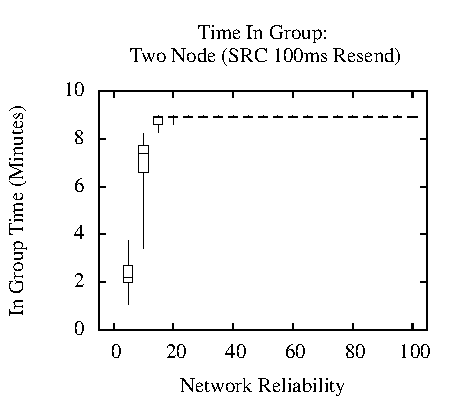
\includegraphics[width=\linewidth]{2NODE-SRC-100-GROUP.pdf}
\caption{Time in group over a 10 minute run for two node system with 100ms resend time}
\label{fig:IGT-SRC-2NODE-100}
\end{figure}

The 100ms resend SRC test with two nodes can be considered a sort of a control.
These tests, pictured in Figure \ref{fig:IGT-SRC-2NODE-100}, highlights the performance of the
SRC protocol, achieving the maximum in-group time of 9 minutes with only 15\%
of datagrams arriving at the receiver. 

\begin{figure}[!h]
\centering
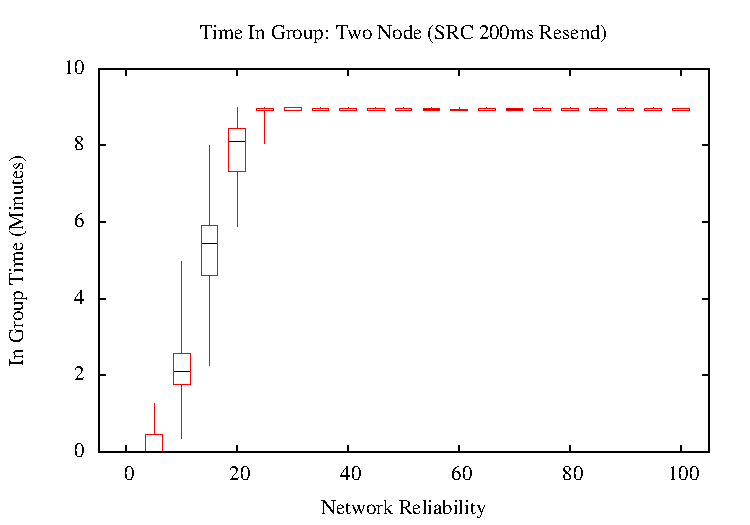
\includegraphics[width=\linewidth]{2NODE-SRC-200-GROUP.pdf}
\caption{Time in group over a 10 minute run for two node system with 200ms resend time}
\label{fig:IGT-SRC-2NODE-200}
\end{figure}

Figures \ref{fig:IGT-SRC-2NODE-200} demonstrates that as the
rate at which lost datagrams are resent is decreased to 200ms the
time in group falls off. This behavior is expected, since each exchange has a
time limit for each message to arrive and the number of attempts is reduced by
increasing the resend time.


\subsubsection{Transient Partition Case}

\begin{figure}[!h]
\centering
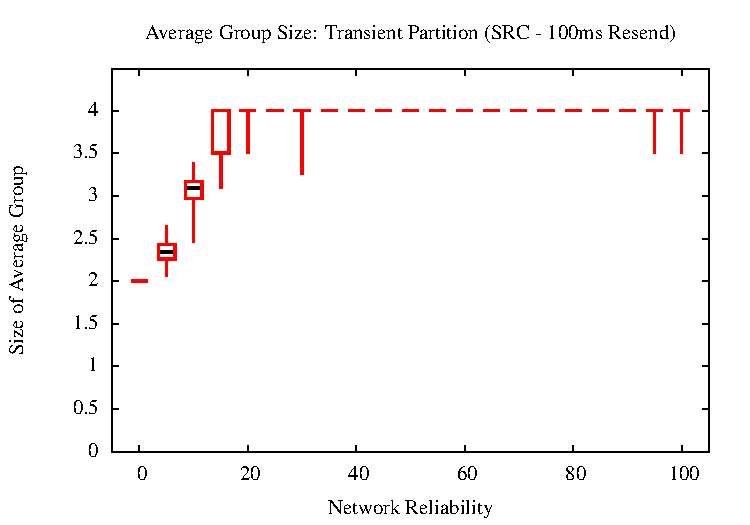
\includegraphics[width=\linewidth]{TRANS-SRC-100-SIZE.pdf}
\caption{Average size of formed groups for the transient partition case with 100ms resend time}
\label{fig:MGS-SRC-TRANS-100}
\end{figure}

\begin{figure}[!h]
\centering
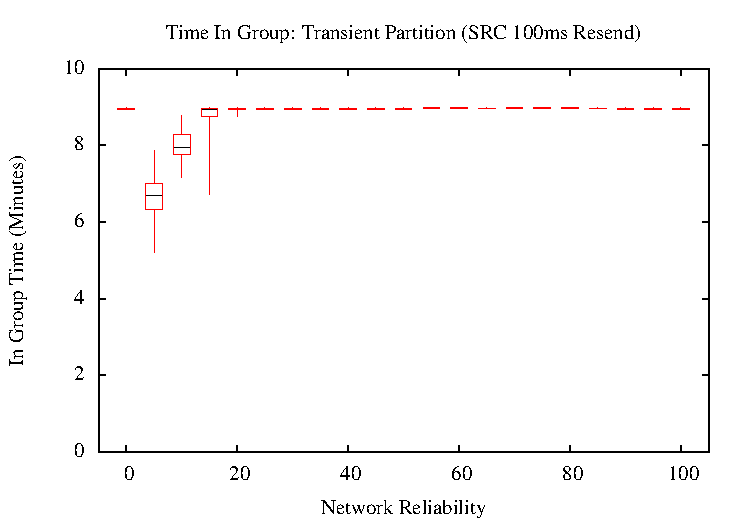
\includegraphics[width=\linewidth]{TRANS-SRC-100-GROUP.pdf}
\caption{Time in group over a 10 minute run for the transient partition case with 100ms resend time}
\label{fig:IGT-SRC-TRANS-100}
\end{figure}

The transient partition case shows a simple example where a network partition
separates two groups of DGI processes. In the simplest case where the opposite side of
the partition is unreachable, nodes will form a group with the other nodes on the
same side of the partition. In our tests, there are two nodes on each side of
the partition. In the experiment, the probability of a datagram crossing the
partition is increased as the experiment continues. The 100ms case is shown in
Figures \ref{fig:MGS-SRC-TRANS-100} and \ref{fig:IGT-SRC-TRANS-100}.

While messages cannot cross the partition, the DGIs stay in a group with the
nodes on the same side of the partition leading to an in group time of 9 minutes,
the maximum value. As packets begin to cross the partition (as the reliability
increases), DGI instances on either side begin to attempt to complete elections
with the nodes on the opposite partition and the time in group begins to fall.
However during this time, the mean group size continues to increase, meaning
while the elections are decreasing the amount of time that the module spends in
state where it can actively do work, it typically does not fall into a state
where it is in a group by itself, which means that most of the lost in-group
time comes from elections.

\begin{figure}[!h]
\centering
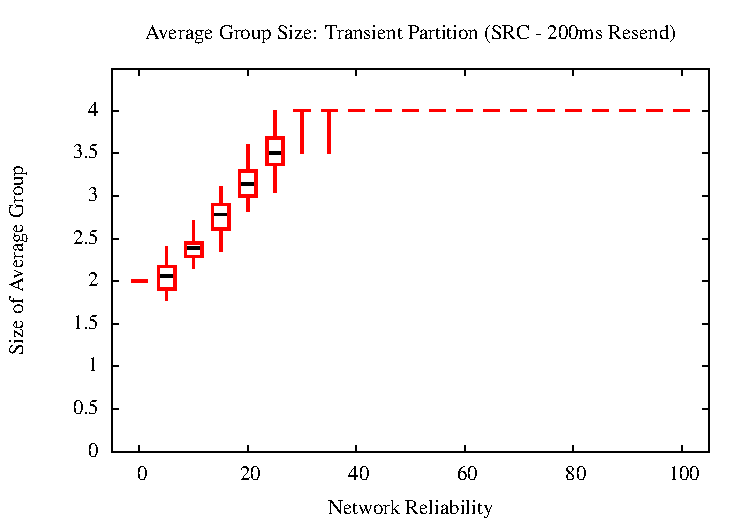
\includegraphics[width=\linewidth]{TRANS-SRC-200-SIZE.pdf}
\caption{Average size of formed groups for the transient partition case with 200ms resend time}
\label{fig:MGS-SRC-TRANS-200}
\end{figure}

\begin{figure}[!h]
\centering
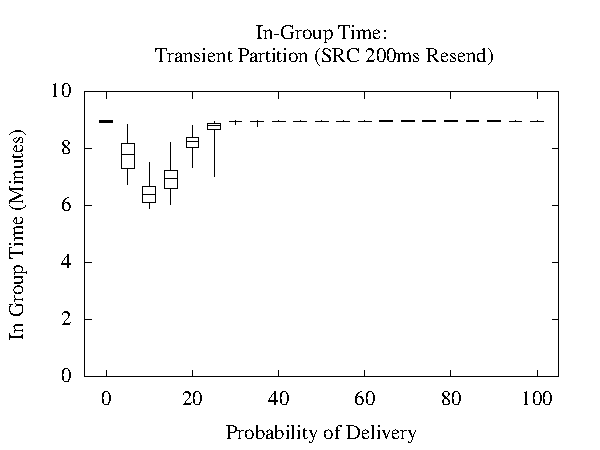
\includegraphics[width=\linewidth]{TRANS-SRC-200-GROUP.pdf}
\caption{Time in group over a 10 minute run for the transient partition case with 200ms resend time}
\label{fig:IGT-SRC-TRANS-200}
\end{figure}

The 200ms case, shown in Figures \ref{fig:MGS-SRC-TRANS-200} and \ref{fig:IGT-SRC-TRANS-200} displays similar behavior, with a wider valley due to the
limited number of datagrams. It is also worth noting the that the mean group
size dips below 2 in the figure, possibly because the longer resend times allow
for more race conditions between potential leaders. Discussion of these race
conditions is shown in discussed during the SUC charts since it is more prevalent
in those experiments.

\subsection{Sequenced Unreliable Connection}

\subsubsection{Two Node Case}

The SUC protocol's experimental tests show an immediate problem: although there
is a general trend of growth in the amount of time in group and group size
charts, shown in Figure \ref{fig:IGT-SUC-2NODE-100}
there is a high amount of variance for any particular trial.

\begin{figure}[!h]
\centering
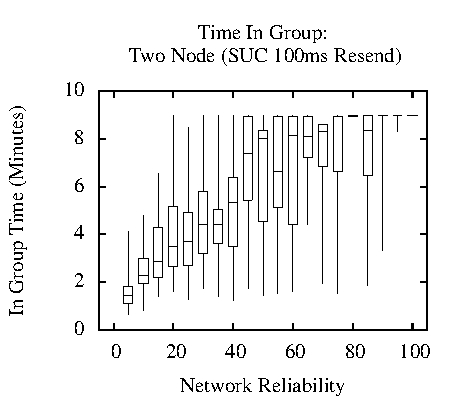
\includegraphics[width=\linewidth]{2NODE-SUC-100-GROUP.pdf}
\caption{Time in group over a 10 minute run for two node system with 100ms resend time}
\label{fig:IGT-SUC-2NODE-100}
\end{figure}

\begin{figure}[!h]
\centering
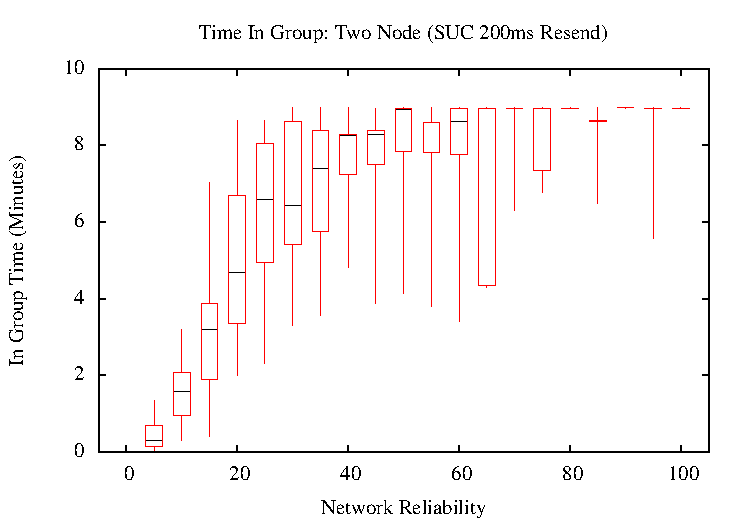
\includegraphics[width=\linewidth]{2NODE-SUC-200-GROUP.pdf}
\caption{Time in group over a 10 minute run for two node system with 200ms resend time}
\label{fig:IGT-SUC-2NODE-200}
\end{figure}

In the 200ms resend case, show in Figure \ref{fig:IGT-SUC-2NODE-200}, it can be 
observed that there is a more growth rate in the in-group time as a the
reliability increases. In fact, averaging across all the collected data points
from the experiment, the average in-group time is higher for the 200ms case
than it is for the 100ms case ( 6.86 vs 6.09 ). However, due to the large amount
of variance in the collected in-group time, it is not possible to state with
confidence that the there is a significant difference between the two cases.

\section{Formal Modeling}

Due to the high amount of variance in the collected data, and the resulting
difficulty making any sort of prediction about other systems from the data, a
more formal approach was tried.

Since the system, taken as a whole, can be reasonably modeled as a collection of 
states each describing the state or configuration of the system, and that the
transitions between those state (failure events or election events) are probabilistic,
rather than deterministic, it is a natural extension to model the distributed
system as a Markov Chain.

\subsection{Assumptions}
In order to model the system, we assumed that the time between events was 
exponentially distributed. Furthermore, we assumed that the system would be
fairly well synchronized, with most elections occurring at the same time. This
assumption was valid for 2-Node cases of our non-real-time code, but was
a major issue as the number of nodes began to increase. However, with of
the use of the round-robin scheduler with synchronization to enforce our
real-time requirements, assuming the synchronization of processes is not a
major leap.

All participating peers are assumed to be on the same schedule: all
peers begin execution of a model simultaneously. This is accomplished using \cite{DCS}.
This work assumes that the clocks are synchronized: even if the network has faulted,
process clocks have not drifted noticeably from their last synchronization. Additionally,
a production system would likely use GPS time synchronization in order to take
certain power system readings \cite{PHASORREADINGS}.

\subsection{Constructing The Markov Chain}

Consider a set of processes, which are linked by some packet based network
protocol. In our experiments we provide two protocols, each with different
delivery characteristics. Under ideal conditions a packet sent by one process
will always be delivered to its destination. Without a delivery protocol, as
soon as packets are lost by the communication network, the message that it
contained is lost forever. Therefore to compensate for the network losing
packets, a large variety of delivery protocols have been adapted. Each protocol
has a different set of goals and objectives, depending on the application.

Keeping in mind that a single lost packet does not necessitate the message it
contained is forever lost, different protocols allow for different levels of
reliability despite packet loss.

The leader election algorithm is centered around two critical events: checking,
and elections. The check system is used to detect both failures and the
availability of nodes for election. Processes in the system occasionally exchange 
messages to determine if the other processes have crashed, and to discover new
leaders. 

The DGI can perform work assuming that it is in a group, and not in an election
state (since the group management module instructs other modules to stop during
an election). The collected data in the previous sections is based on that
assumption, and the Markov chains that models those scenarios needed to as
well.

Processes in the DGI are either members or leaders. Leaders are processes
which have won elections among its members.

As stated previously, it was assumed that the events in the distributed system
were distributed exponentially. Events are modeled in the chain
using $\lambda(x)$ which is the parameter of the exponential distribution. It
is important to note that:

\begin{equation}
\mathrm{E}[X] = \frac{1}{\lambda}. \!
\end{equation}

and

\begin{equation}
\lambda(x) = \sum \lambda(x,y) = \sum \lambda(x) p(x,y)
\end{equation}

Where $\lambda(x)$ is the exponential parameter for the total time spend in
a state $x$, $\lambda(x,y)$ is the exponential parameter for a transition from
state $x$ to state $y$, and $p(x,y)$ is the normally distributed probability that
a state transitions from state $x$ to state $y$.

\subsubsection{Failure Detection}
When a leader sends its check messages, the nodes that receive it either
respond in the positive, indicating that they are also leaders, or in the
negative indicating that they have already joined a group. This message is sent
to all known nodes in the system. If a process replies that it is also a
leader, the original sender will enter and election mode and attempt to combine
groups with the first process. Nodes that fail to respond are removed from the
leaders group, if they were members.

The member on the other hand will only direct its check message to the leader
of its current group. As with the leader's check message, the response can
either be positive or negative. A ``yes'' response indicates that the leader is
still available and considers the member a part of its group. A ``no'' response
indicates that either the leader has failed and recovered, or it has suspected
the member process of being unreachable (either due to crash or network issue)
and has removed them from the group. In this event the member will enter a
recovery state and reset itself to an initial configuration where it is in a
group by itself.

On any membership change, either due to recovery, or a suspected failure, the
list of members for a group is pushed to every member of that group by the
leader. Members cannot suspect other processes of being crashed, only the
leader can identify failed group members.

\begin{figure}
\centering
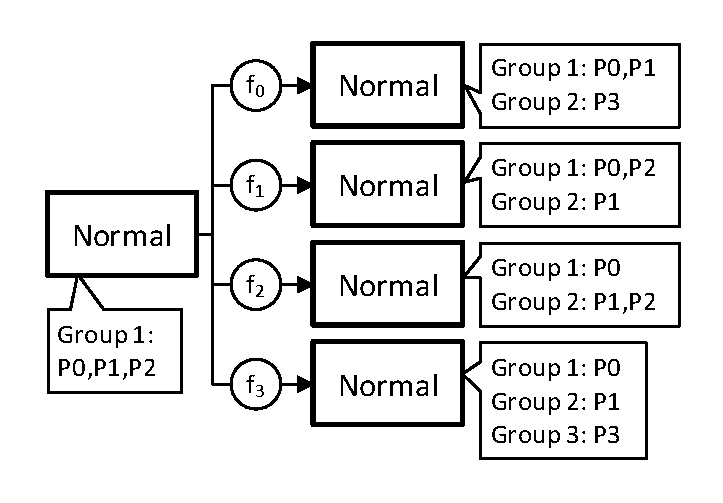
\includegraphics[width=.9\linewidth]{MarkovAYC2.pdf}
\caption{A diagram showing a partial Markov chain for failure detection}
\label{fig:MARKOVAYC}
\end{figure}

A model of a failure detection stage of the leader election algorithm is presented in
Figure \ref{fig:MARKOVAYC}. A set of nodes begin in a normal state as part of a group.
The leader sends a query to every member, and every member sends a query to the leader.
If a response is not received in either direction, the process is considered to be
unreachable and is either ejected from the group by the leader (if the query originated from the leader)
or the member leaves the group and becomes a coordinator themselves.

The system will stay in the original state as long as all nodes complete their queries and responses.
Let $T_{R}$ be the amount of time allowed for a response, $T_{C}$ be the time between
discovery attempts, and $p_{F}$ is the probability that at least one peer fails to complete the exchange.
Based on this, the expected amount of time in the grouped state ($T_{G}$) is:

\begin{equation}
\begin{cases}
T_{G} = ( T_{R}+T_{C}  ) / p_{F} & p_{F} > 0 \\
\infty & p_{F} = 0
\end{cases}
\end{equation}

Let $\delta$ equal exponential parameter of the exponential distribution for the base state. Then
we can relate the probabilities of each possible transition to the parameter for the base state. Let
$p_{i}$ be the probability of transitioning to configuration $i$ after leaving the base state and let
$f_{i}$ be the exponential parameter for the transition to an individual configuration:

\begin{equation}
\delta = \sum f_{i} = \sum \delta p_{i} = \frac{1}{T_{G}}
\end{equation}


\subsubsection{Leader Election}
During elections, a highest priority leader (identified by its process id) will
send invites to the other leaders it has identified. If those leaders accept
the highest priority leader's invites, they will reply with an accept message
and forward the invite to their members, if their are any. If the highest
priority process fails to become the leader the next highest will send invites
after a specified interval has passed.

Therefore, the membership of the system can be affected in two ways: election
events which change the size of groups and failure suspicion (via checks) which
decreases the size of groups. Note that elections can decrease the size of
groups as well as increase them: If a round of forwarding invites fails by the
new leader to his original group, the group size could decrease.

When a process is initialized it begins in the ``solo'' state: it is in a group
with itself as the only member. As nodes are discovered by checks, the
processes combine into groups. Groups are not limited by increasing one a time;
they can increase by combined size of the groups of the leader processes.

We define a metric to assess the performance of the system under duress: we
first consider that the distributed can only perform meaningful work when the
processes can work together to perform physical migration. This means that
there are two networks that affect the system's ability to do work: the
physical flow network and the cyber communication network.


\begin{figure*}
\centering
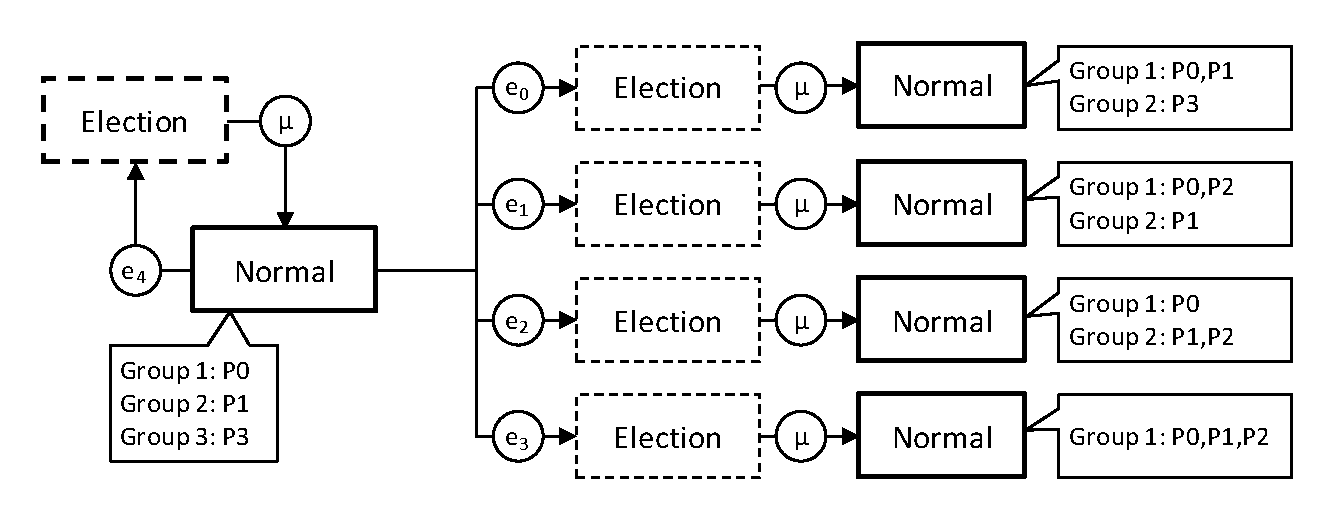
\includegraphics[width=1.0\linewidth]{MarkovElection2.pdf}
\caption{A diagram showing a partial Markov chain for an election}
\label{fig:MARKOVELECTION}
\end{figure*}

A continuous time Markov model of a single election is presented in Figure \ref{fig:MARKOVELECTION}.
A set of leaders begin in a normal state. After some time $T_{D}$ an ``are you coordinator''
message discovers some other peer. $T_{D}$ is a function of the number of discovery
checks which discover no leaders (which in turn is a function of the link reliability). Let
$T_{R}$ be the amount of time allowed for a response, $T_{C}$ be the time between
discovery attempts, and $p_{D}$ is the probability that the exchange discovers a leader.

\begin{equation}
\begin{cases}
T_{D} = ( T_{R}+T_{C} ) / p_{D} & p_{D} > 0 \\
\infty & p_{D} = 0
\end{cases}
\end{equation}

Then, the parameters $e_x$ in Figure \ref{fig:MARKOVELECTION} are a function of $T_{D}$ and $p_{x}$,
the probability an election results in configuration $x$.

\begin{equation}
e_x = \frac{p_{x}}{T_{D}}
\end{equation}

Once a leader has been discovered, the system transitions into an election state, based on the
potential outcome, where the peers hold an election to determine a new configuration. As shown
in Figure \ref{fig:MARKOVELECTION}, an election can either succeed or fail, resulting in a new system
configuration, or each involved process to return to the single member group state.
 
The amount of time that an election takes is fixed before the algorithm is executed. 
Let $T_{E}$ be the mean time it takes to complete any election. Therefore:

\begin{equation}
\mu = \frac{1}{T_{E}}
\end{equation}

\subsubsection{Combined Model}

A combined model combines election and failure detection Markov chain components. Except for the
states where all reachable nodes are in the same group and the states where there are no reachable
leaders each state has a combination of election transitions and failure transitions.                                                        
The combined model is predictive of the overall characteristics of the system. The
time spent in a particular configuration is a function of the $\lambda$'s of all the
events that can cause the system to transition away from a configuration. 

To construct the Markov chain, simulations of individual events are performed. The circumstances
for the events are assumed to be homogeneous: processes only differ by their process id.
Using this assumption, the simulation of events can be broken down into a series of scenarios
that are representative of the events in the system. Since each scenario is independent of other
scenarios, each scenario can be run independently.  Additionally, since the circumstances
are assumed to be homogeneous, scenarios that are similar, such as ones where two processes
swap roles can be simulated only once, and the results can be transformed from one scenario
to another with a simple mapping. This mapping scheme and parallizability helps keep the
state space explosion of the potential states under control.

\section{Model Calibration}

The presented methodology of constructing the model was initially calibrated against the
original two-node case, using a non-real-time version of the DGI codebase. The resulting
Markov chain was processed using SharpE \cite{SHARPE}\cite{SHARPE2} made by Dr. Kishor
Trivedi's group at Duke University, a popular tool for reliability analysis. SharpE measured the reward collected in 600 seconds,
minus the reward that was collected in the first 60 seconds (to emulate that the first
60 seconds were discarded in the experimental runs.) The SharpE results are plotted along
with the experimental results in Figures \ref{fig:COMPARE-SUC-2NODE-100} and \ref{fig:COMPARE-SUC-2NODE-200}.

\begin{figure}[!h]
\centering
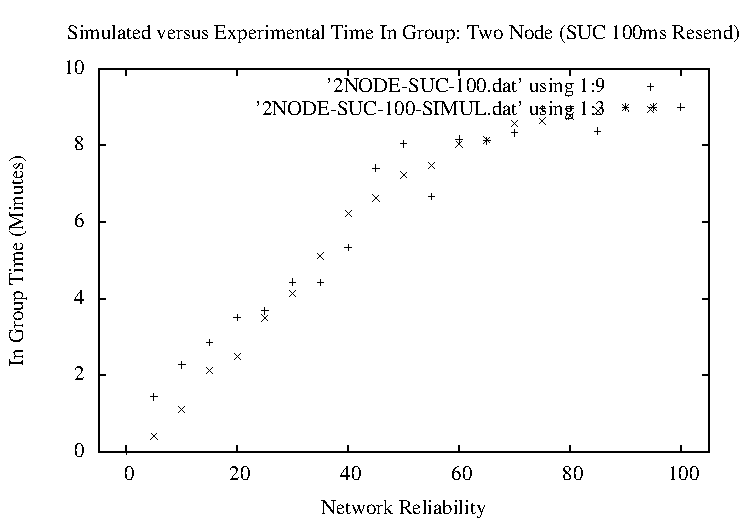
\includegraphics[width=1.0\linewidth]{2NODE-SUC-100-COMPARE.pdf}
\caption{Comparison of in-group time as collected from the experimental platform and the simulator (1 tick offset between processes).}
\label{fig:COMPARE-SUC-2NODE-100}
\end{figure}


\begin{figure}[!h]
\centering
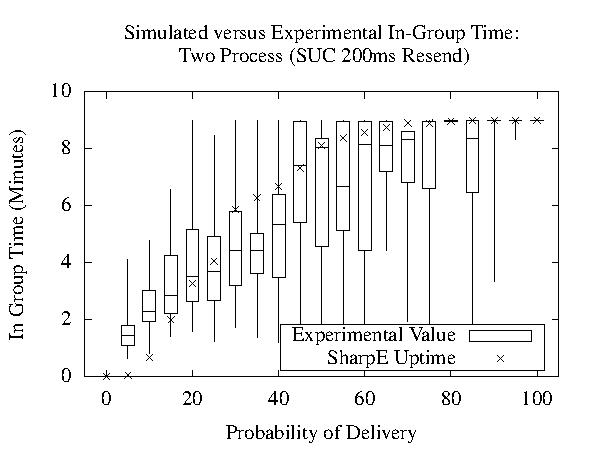
\includegraphics[width=1.0\linewidth]{2NODE-SUC-200-COMPARE.pdf}

\caption{Comparison of in-group time as collected from the experimental platform and the simulator (2 tick offset between processes).}
\label{fig:COMPARE-SUC-2NODE-200}
\end{figure}

The race condition between processes during an election is a consideration in the original
leader election algorithm, and is an additional factor here. The simulator provided a parameter
to allow the operator to select how closely synchronized the peers were (the time difference
between when each of them would search for leaders.) The exchange of messages, particularly
during an election had a tendency to synchronize nodes during elections, and so the nodes could
synchronize even if they did not initially begin in a synchronized state. As a result, the
simulation results aligned best for the 100ms resend case with 1 ticks (Approximately 100ms
difference in synchronization between processes) and 2 ticks (Approximately 400ms) in the 200ms
resend case.

Models fit to the non-real-time code in groups larger than 2 processes did not fit well.
This is presumed to be a combination of several factors. The suspected major source of fault
included the structure of the chain, which naturally assumes that all processes enter the
election state a roughly the same time, which is not typically true for any number of processes
greater than 2. Additionally, the simulator could only assume that the synchronization between
processes was mostly fixed, which was not the case in the larger configurations, since the
coincidental synchronization that occurred in the two node case was suppressed by the increased
number of peers. Furthermore, an issue with SharpE was discovered that prevented the
particular structure of the chains produced from being handled correctly. To circumvent that,
issue, SharpE was replaced by a random-walker which generates exponentially distributed numbers
and follows the paths of the chain, across several hundred trials, in order to collect time in group data for
models which SharpE cannot process.

The structure of the Markov Chain, which assumed that processes enter the election state
mostly simultaneously was an appropriate assumption for the real-time system, since the
round-robin scheduler synchronizes when processes run their group management modules. The
simulator was set to assume that the synchronization between processes was very tight, and
new experimental data was collected for the 4 node, transient partition case. The collected
data is overlaid with the results from the random walker in Figures \ref{fig:COMPARE-SUC-TRANS-RT-128} and \ref{fig:COMPARE-SUC-TRANS-RT-64}.

\begin{figure}[!h]
\centering
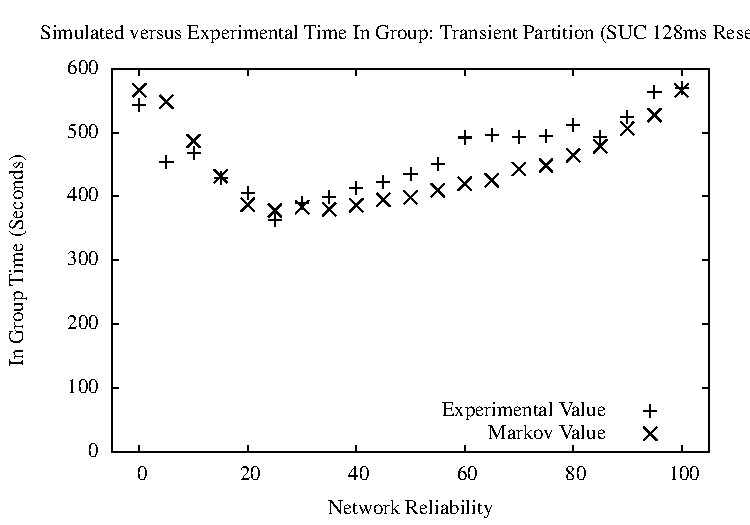
\includegraphics[width=1.0\linewidth]{TRANS-RT-SUC-128-COMPARE.pdf}

\caption{Comparison of in-group time as collected from the experimental platform and the time in group from the equivalent Markov chain (128ms between resends).}
\label{fig:COMPARE-SUC-TRANS-RT-128}
\end{figure}

\begin{figure}[!h]
\centering
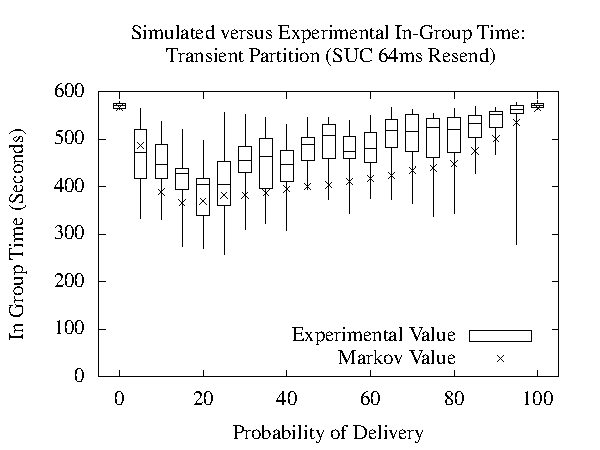
\includegraphics[width=1.0\linewidth]{TRANS-RT-SUC-64-COMPARE.pdf}

\caption{Comparison of in-group time as collected from the experimental platform and the time in group from the equivalent Markov chain (64ms between resends).}
\label{fig:COMPARE-SUC-TRANS-RT-64}
\end{figure}

As a measure of the strength of the model, the correlation between the predicted value was compared.
The average error was also computed for each of the samples taken. This information is presented in
Table \ref{tab:STAT-DATA}.

\begin{table}
% increase table row spacing, adjust to taste
\caption{Error and correlation of experimental data and Markov chain predictions}
\label{tab:STAT-DATA}
\centering
% Some packages, such as MDW tools, offer better commands for making tables
% than the plain LaTeX2e tabular which is used here.
\begin{tabular}{|c||c|c|c|} 
\hline
Resend & Correlation & Error \\ \hline
128 & 0.7656 & 11.61\% \\ \hline
64 & 0.8604 & 11.70\% \\ \hline 
\end{tabular}
\end{table}

% An example of a floating figure using the graphicx package.
% Note that \label must occur AFTER (or within) \caption.
% For figures, \caption should occur after the \includegraphics.
% Note that IEEEtran v1.7 and later has special internal code that
% is designed to preserve the operation of \label within \caption
% even when the captionsoff option is in effect. However, because
% of issues like this, it may be the safest practice to put all your
% \label just after \caption rather than within \caption{}.
%
% Reminder: the "draftcls" or "draftclsnofoot", not "draft", class
% option should be used if it is desired that the figures are to be
% displayed while in draft mode.
%
%\begin{figure}[!t]
%\centering
%\includegraphics[width=2.5in]{myfigure}
% where an .eps filename suffix will be assumed under latex, 
% and a .pdf suffix will be assumed for pdflatex; or what has been declared
% via \DeclareGraphicsExtensions.
%\caption{Simulation Results}
%\label{fig_sim}
%\end{figure}

% Note that IEEE CS typically puts floats only at the top, even when this
% results in a large percentage of a column being occupied by floats.
% However, the Computer Society has been known to put floats at the bottom.


% An example of a double column floating figure using two subfigures.
% (The subfig.sty package must be loaded for this to work.)
% The subfigure \label commands are set within each subfloat command, the
% \label for the overall figure must come after \caption.
% \hfil must be used as a separator to get equal spacing.
% The subfigure.sty package works much the same way, except \subfigure is
% used instead of \subfloat.
%
%\begin{figure*}[!t]
%\centerline{\subfloat[Case I]\includegraphics[width=2.5in]{subfigcase1}%
%\label{fig_first_case}}
%\hfil
%\subfloat[Case II]{\includegraphics[width=2.5in]{subfigcase2}%
%\label{fig_second_case}}}
%\caption{Simulation results}
%\label{fig_sim}
%\end{figure*}
%
% Note that often IEEE CS papers with subfigures do not employ subfigure
% captions (using the optional argument to \subfloat), but instead will
% reference/describe all of them (a), (b), etc., within the main caption.


% An example of a floating table. Note that, for IEEE style tables, the 
% \caption command should come BEFORE the table. Table text will default to
% \footnotesize as IEEE normally uses this smaller font for tables.
% The \label must come after \caption as always.
%
%\begin{table}[!t]
%% increase table row spacing, adjust to taste
%\renewcommand{\arraystretch}{1.3}
% if using array.sty, it might be a good idea to tweak the value of
% \extrarowheight as needed to properly center the text within the cells
%\caption{An Example of a Table}
%\label{table_example}
%\centering
%% Some packages, such as MDW tools, offer better commands for making tables
%% than the plain LaTeX2e tabular which is used here.
%\begin{tabular}{|c||c|}
%\hline
%One & Two\\
%\hline
%Three & Four\\
%\hline
%\end{tabular}
%\end{table}


% Note that IEEE does not put floats in the very first column - or typically
% anywhere on the first page for that matter. Also, in-text middle ("here")
% positioning is not used. Most IEEE journals use top floats exclusively.
% However, Computer Society journals sometimes do use bottom floats - bear
% this in mind when choosing appropriate optional arguments for the
% figure/table environments.
% Note that, LaTeX2e, unlike IEEE journals, places footnotes above bottom
% floats. This can be corrected via the \fnbelowfloat command of the
% stfloats package.



\section{Conclusion}

This work presented a new approach for predicting the behavior of a real-time
distributed system under omission failure conditions. By using a continuous time
Markov chain, a variety of insights can be gathered about the system, including
observations such as how long a particular configuration will be stable for, 
and the behavior of the system in the long run.  The Markov results will be used
 to make better real time schedules to better react to the network faults we
plan on introducing to our testbeds. For example, if migrations are failing
and a sufficient number of migrations can cause the physical system to fail,
the scheduler may need to behave in a manner that limits the number of failed
migrations that can occur before group reconfigures. This work is a stepping
stone towards designing a real-time schedule that manages the system correctly
when there are cyber faults. Schedules and behavior can be designed around how
the system behaves on its worst days. This work also allows these schedule designs
and evaluations to be completed much more quickly than they could be by running
the system for long periods of time. Therefore results from the test bed, combined
with results the models yield schedules that improve the stability of the
system during cyber faults.


% if have a single appendix:
%\appendix[Proof of the Zonklar Equations]
% or
%\appendix  % for no appendix heading
% do not use \section anymore after \appendix, only \section*
% is possibly needed

% use appendices with more than one appendix
% then use \section to start each appendix
% you must declare a \section before using any
% \subsection or using \label (\appendices by itself
% starts a section numbered zero.)
%


% use section* for acknowledgement
\ifCLASSOPTIONcompsoc
  % The Computer Society usually uses the plural form
  \section*{Acknowledgments}
\else
  % regular IEEE prefers the singular form
  \section*{Acknowledgment}
\fi
The authors acknowledge the support of the Future Renewable
Electric Energy Delivery and Management Center,
a National Science Foundation supported Engineering Research
Center under grant NSF EEC-081212, and the United States Department of Education GAANN program.

% Can use something like this to put references on a page
% by themselves when using endfloat and the captionsoff option.
\ifCLASSOPTIONcaptionsoff
  \newpage
\fi



% trigger a \newpage just before the given reference
% number - used to balance the columns on the last page
% adjust value as needed - may need to be readjusted if
% the document is modified later
%\IEEEtriggeratref{8}
% The "triggered" command can be changed if desired:
%\IEEEtriggercmd{\enlargethispage{-5in}}

% references section

% can use a bibliography generated by BibTeX as a .bbl file
% BibTeX documentation can be easily obtained at:
% http://www.ctan.org/tex-archive/biblio/bibtex/contrib/doc/
% The IEEEtran BibTeX style support page is at:
% http://www.michaelshell.org/tex/ieeetran/bibtex/
\bibliographystyle{IEEEtran}
% argument is your BibTeX string definitions and bibliography database(s)
\bibliography{IEEEabrv,latex_bibliography}
%
% <OR> manually copy in the resultant .bbl file
% set second argument of \begin to the number of references
% (used to reserve space for the reference number labels box)

%This is an example of a Transactions article reference
%D.S. Coming and O.G. Staadt, "Velocity-Aligned Discrete Oriented Polytopes for Dynamic Collision Detection," IEEE Trans. Visualization and Computer Graphics, vol.�14,� no.�1,� pp. 1-12,� Jan/Feb� 2008, doi:10.1109/TVCG.2007.70405.

%This is an example of a article from a conference proceeding
%H. Goto, Y. Hasegawa, and M. Tanaka, "Efficient Scheduling Focusing on the Duality of MPL Representation," Proc. IEEE Symp. Computational Intelligence in Scheduling (SCIS '07), pp. 57-64, Apr. 2007, doi:10.1109/SCIS.2007.367670.

%This is an example of a PrePrint reference
%J.M.P. Martinez, R.B. Llavori, M.J.A. Cabo, and T.B. Pedersen, "Integrating Data Warehouses with Web Data: A Survey," IEEE Trans. Knowledge and Data Eng., preprint, 21 Dec. 2007, doi:10.1109/TKDE.2007.190746.

%Again, see the IEEEtrans_HOWTO.pdf for several more bibliographical examples. Also, more style examples
%can be seen at http://www.computer.org/author/style/transref.htm

% biography section
% 
% If you have an EPS/PDF photo (graphicx package needed) extra braces are
% needed around the contents of the optional argument to biography to prevent
% the LaTeX parser from getting confused when it sees the complicated
% \includegraphics command within an optional argument. (You could create
% your own custom macro containing the \includegraphics command to make things
% simpler here.)
%\begin{biography}[{\includegraphics[width=1in,height=1.25in,clip,keepaspectratio]{mshell}}]{Michael Shell}
% or if you just want to reserve a space for a photo:

\begin{IEEEbiography}{Stephen Jackson}
Received a BS in Computer Engineering and Computer Science from Missouri University of Science \& Technology in 2010. He is currently pursuing a PhD in Computer Science at Missouri S\&T. He is a member of the Critical Infrastructure Protection Laboratory at S\&T, and a recipient of the Information-Assurance GAANN fellowship. His research interests include distributed systems, cyber-physical systems, and system reliability.
\end{IEEEbiography}

% if you will not have a photo at all:
\begin{IEEEbiography}[{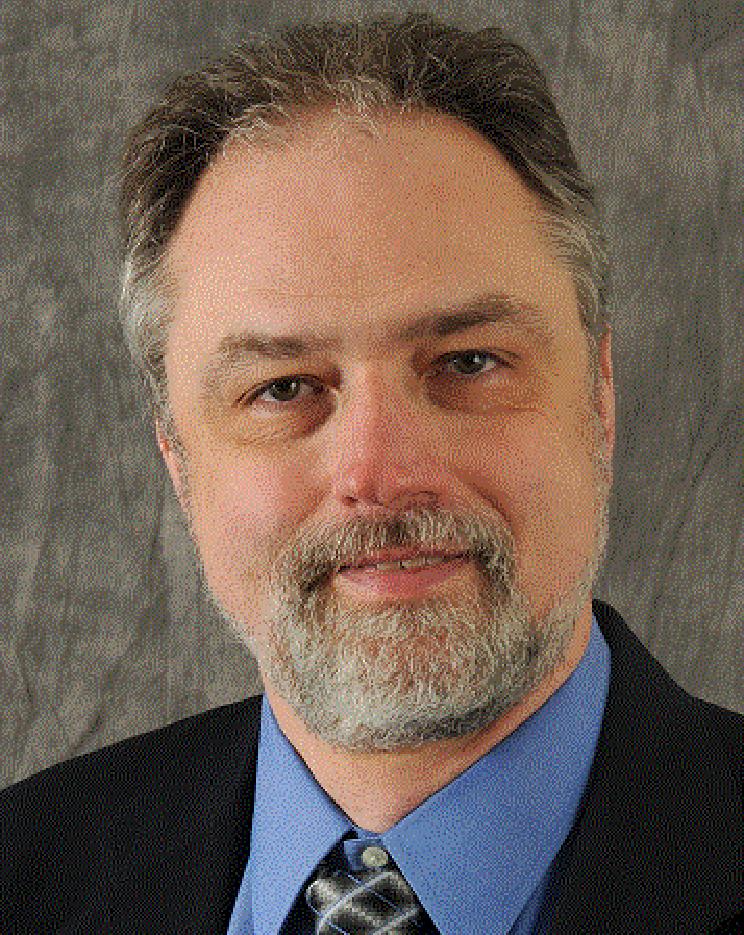
\includegraphics[width=1in,height=1.25in,clip,keepaspectratio]{bmcmillin}}]{Bruce McMillin}
 (SM '07) is currently a Professor
of Computer Science and Director of the Center for
Information Assurance at Missouri S\&T, Rolla, MO,
USA. He leads and participates in interdisciplinary
teams in formal methods for fault tolerance and security
in distributed embedded systems with an eye towards
critical infrastructure protection. He is leading
the distributed grid intelligence project of the Future
Renewables Engineering Research Center.
\end{IEEEbiography}

% insert where needed to balance the two columns on the last page with
% biographies
%\newpage

% You can push biographies down or up by placing
% a \vfill before or after them. The appropriate
% use of \vfill depends on what kind of text is
% on the last page and whether or not the columns
% are being equalized.

\vfill

% Can be used to pull up biographies so that the bottom of the last one
% is flush with the other column.
%\enlargethispage{-5in}



% that's all folks
\end{document}



